\documentclass[11pt]{article}
\usepackage[utf8]{inputenc}
\usepackage[T1]{fontenc}
\usepackage[margin=1in]{geometry}
\usepackage{graphicx}
\usepackage{booktabs}
\usepackage{array}
\usepackage{hyperref}
\usepackage{float}
\usepackage{amsmath}
\usepackage{enumitem}
\usepackage{xcolor}
\hypersetup{colorlinks=true, linkcolor=blue, urlcolor=blue, hypertexnames=false}
\definecolor{AccentBlue}{HTML}{1F4E79}
\definecolor{SoftBlue}{HTML}{EFF6FF}
\definecolor{SoftGreen}{HTML}{ECFDF5}
\definecolor{RuleGray}{HTML}{D0D7DE}
\setlength{\parindent}{0pt}
\setlength{\parskip}{0.45em}
\newcommand{\reportnote}[2]{%
\begin{center}
\fcolorbox{RuleGray}{#1}{%
\begin{minipage}{0.92\linewidth}
#2
\end{minipage}}
\end{center}}

\title{Prédiction de l'entrée en zone dangereuse par vision fixe}
\author{El Fahime Mohamed Zayd \and Bensaid Ilyas \\ Supervised by: Prof. Tawfik Masrour}
\date{Mai 2026}

\begin{document}
\maketitle

\begin{abstract}
Ce rapport résume un prototype académique de sécurité machine à caméra fixe. La tâche principale est de prédire, à partir des images déjà vues, si une partie du corps va entrer dans un volume dangereux annoté. Le système est présenté avec deux usages distincts: un signal court horizon pour l'arrêt automatique, et des signaux plus précoces pour l'alerte opérateur. Les modèles d'attention et de blouse/PPE ne sont pas présentés comme une fusion causale apprise avec le danger physique; ils servent seulement à modifier la politique d'alerte.
\end{abstract}

\section{Introduction}
La sécurité autour d'une machine ne se résume pas à détecter qu'un accident est déjà arrivé. Dans un atelier réel, le système utile est celui qui donne quelques centaines de millisecondes d'avance: assez tôt pour prévenir un technicien, ou assez fiable pour déclencher une chaîne d'arrêt quand l'entrée dans la zone dangereuse devient imminente. Ce projet étudie cette question dans un cadre volontairement limité et contrôlé: une caméra fixe, une machine, une zone dangereuse annotée, et des gestes filmés avec deux acteurs.

La question de recherche est la suivante: dans quelle mesure une caméra fixe, couplée à un modèle vidéo causal, peut-elle anticiper l'entrée physique d'une partie du corps dans une zone dangereuse afin de donner soit un avertissement exploitable au technicien, soit une courte marge d'action à la machine pour initier un arrêt automatique?

Cette question est évaluée sous une contrainte causale stricte: à l'instant $t$, le modèle ne voit que les images disponibles jusqu'à $t$. La cible quantitative reste l'entrée physique dans le volume dangereux, tandis que les annotations de risque visible humain servent de repère qualitatif pour juger si l'alerte arrive à un moment comparable à ce qu'un technicien ou un responsable sécurité pourrait percevoir.

\reportnote{SoftBlue}{\textbf{Point méthodologique.} Les chiffres de performance doivent être lus avec les choix de vérité terrain et de split: l'entrée physique définit la cible quantitative, tandis que le risque visible humain sert de repère d'anticipation.}

\section{Objectifs opérationnels}
\begin{itemize}[leftmargin=*]
\item \textbf{Arrêt automatique.} Utiliser seulement un signal très proche, très confiant, autour de $0,2$--$0,3$ s. Ce signal est trop rapide pour une réaction humaine; il sert à déclencher une chaîne électronique et mécanique.
\item \textbf{Alerte opérateur.} Utiliser un score unique de risque visible maintenant, puis mesurer après coup son avance réelle avant l'entrée. Une alerte peut être plus sensible qu'un arrêt automatique.
\item \textbf{Attention et blouse/PPE.} Ces modèles augmentent la sensibilité de l'alerte quand l'opérateur regarde ailleurs ou porte mal la blouse. Ce n'est pas une preuve que ces variables causent l'entrée dans notre petit dataset.
\end{itemize}

Ces trois usages n'ont pas le même niveau de risque acceptable. Une alerte humaine peut tolérer davantage de faux positifs si elle arrive tôt. Un arrêt automatique doit au contraire être plus conservateur et reposer sur un signal court horizon très confiant. Cette séparation guide toute la suite du rapport.

\reportnote{SoftGreen}{\textbf{Contributions principales.} Le projet apporte: (1) un outil d'annotation adapté à la zone dangereuse et au risque visible; (2) une représentation causale pose-zone avec vitesse et accélération; (3) un score unique de risque visible maintenant, évalué par son avance réelle avant l'entrée physique; (4) une couche de politique qui utilise attention et blouse/PPE comme modificateurs de sensibilité, pas comme preuve directe de danger physique.}

\section{Données, annotations et vérité terrain}
Le dataset contient 72 vidéos parentes, filmées avec la même caméra fixe, la même machine et le même environnement. Les annotations actuelles contiennent 50 entrées physiques dans le volume dangereux, 13 presque-accidents et 9 clips sans danger.

Cette répartition doit être lue comme un comptage d'épisodes, pas comme un comptage du temps observé. Les clips sans danger et les portions avant/après événement fournissent beaucoup de temps négatif: dans le dataset séquentiel principal, on obtient 4\,100 fenêtres issues de clips non dangereux contre 864 fenêtres issues de clips d'entrée, et pour la cible à $1,0$ s seulement 388 fenêtres positives contre 4\,576 négatives. Le choix d'avoir beaucoup d'épisodes d'entrée est volontaire: l'entrée dans le volume est l'événement rare mais critique à apprendre, tandis que le temps sans entrée reste largement présent au niveau des fenêtres d'entraînement.

Les vidéos brutes sont classées par scénario de tournage, puis revues dans l'outil d'annotation. L'annotation produit la zone dangereuse, les segments attention/blouse et les événements temporels. Les scripts de préparation transforment ensuite ces éléments en fenêtres causales d'entraînement, en crops personne, puis en splits train/validation/test par vidéo parente.

\begin{table}[H]
\centering
\caption{Granularité du dataset. Tous les échantillons dérivés gardent le split de leur vidéo parente.}
\begin{tabular}{lrrrr}
\toprule
Artefact & Échantillons & Vidéos parentes & Train & Val/Test \\
\midrule
Vidéos parentes & 72 & 72 & 50 & 11/11 \\
Fenêtres temporelles & 4585 & 66 & 3290 & 799/496 \\
Images crop personne & 712 & 72 & 517 & 92/103 \\
Sous-clips évalués & 1036 & 66 & 738 & 178/120 \\
\bottomrule
\end{tabular}
\end{table}

\begin{figure}[H]
\centering
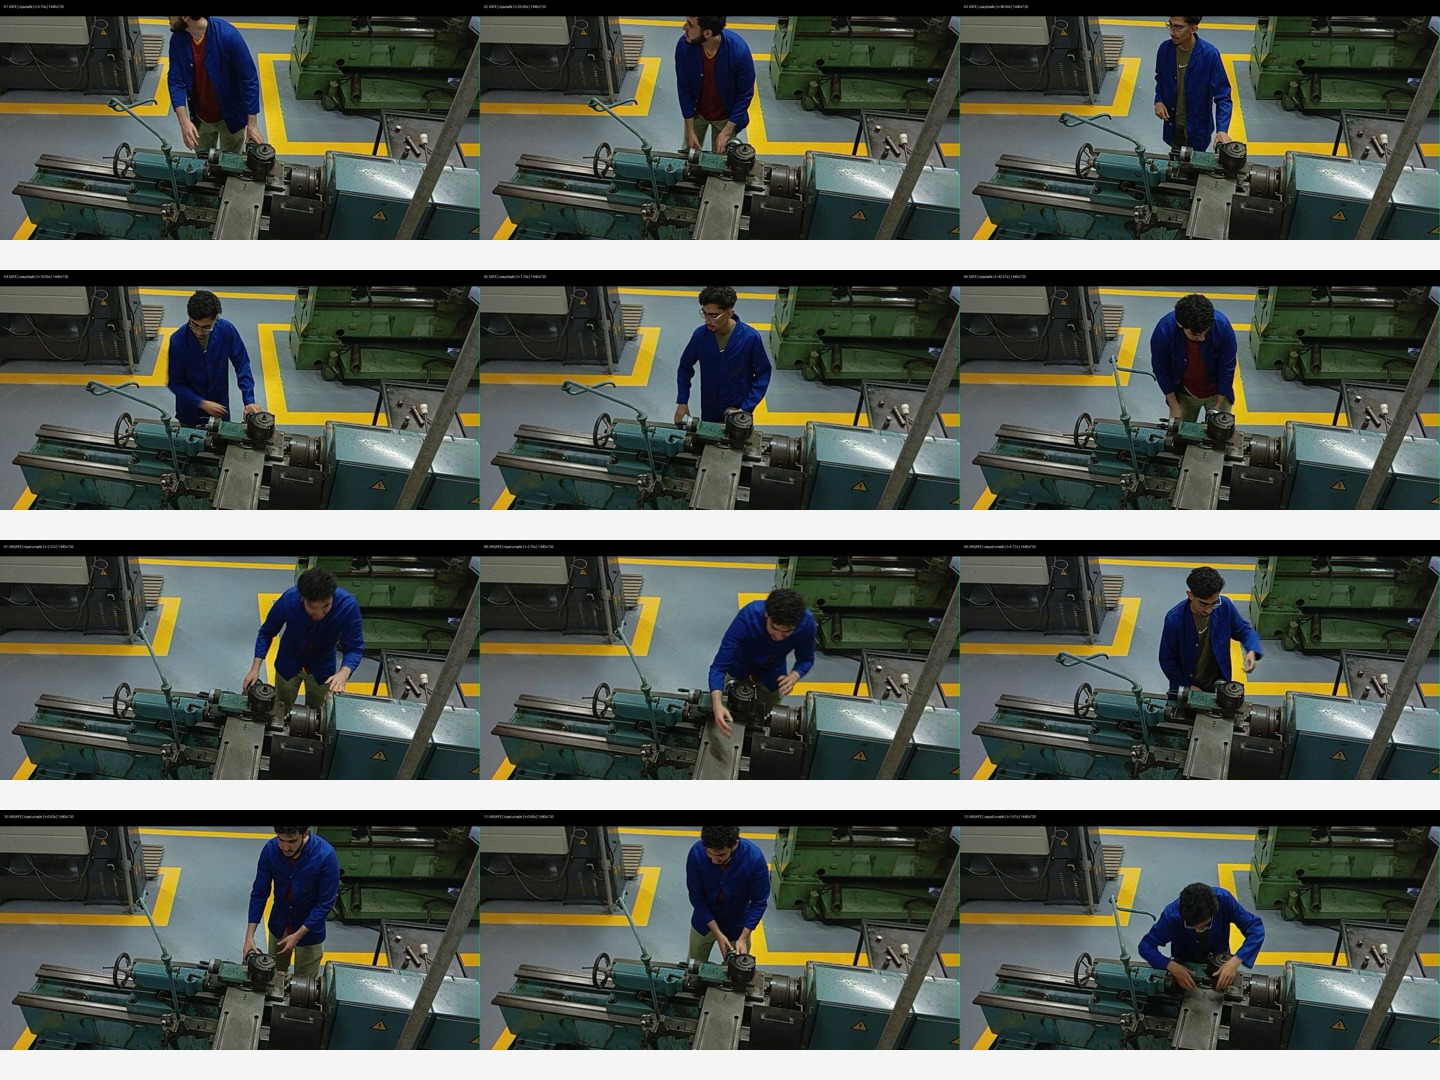
\includegraphics[width=0.92\linewidth]{figures/dataset_montage.jpg}
\caption{Exemples visuels du dataset. La caméra fixe rend le prototype cohérent, mais limite la généralisation.}
\end{figure}

\begin{figure}[H]
\centering
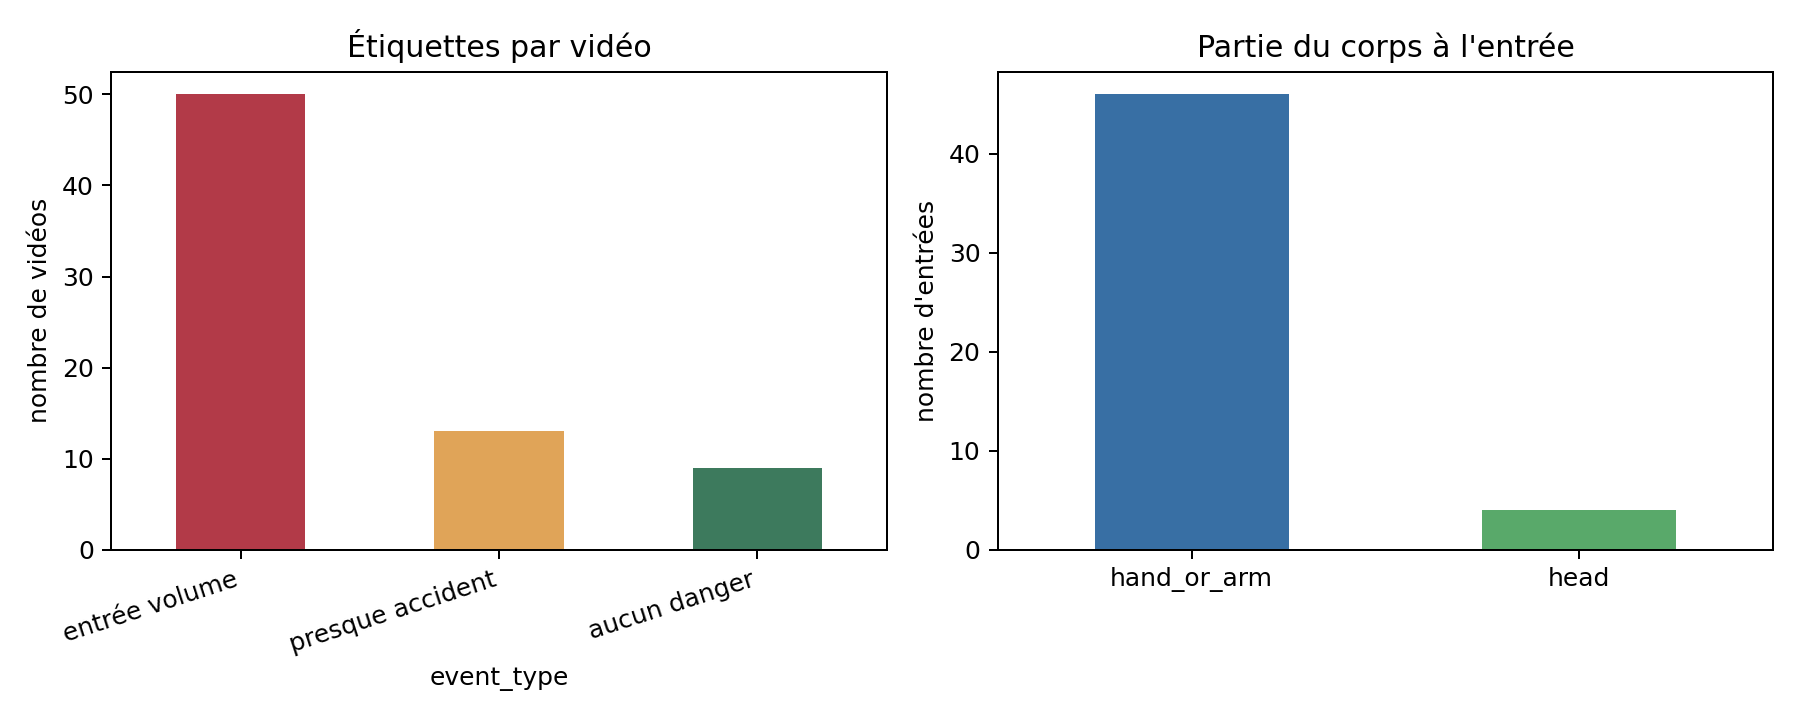
\includegraphics[width=0.85\linewidth]{figures/dataset_event_distribution.png}
\caption{Distribution par vidéo parente. Le graphique compte les épisodes annotés, pas la durée totale ni le nombre de fenêtres: les clips sans danger contribuent beaucoup de temps négatif malgré leur plus faible nombre de vidéos.}
\end{figure}

\subsection{Protocole d'annotation et outil développé}
L'annotation a été traitée comme une partie de la méthode, pas comme une simple étape de rangement des fichiers. Le nom de dossier \texttt{safe} ou \texttt{unsafe} ne suffit pas pour entraîner un système d'alerte précoce: il faut distinguer le moment où un humain compétent peut déjà voir un risque crédible, et le moment objectif où une partie du corps entre réellement dans le volume dangereux. Nous avons donc développé notre propre outil d'annotation pour mesurer ces deux instants dans la même interface.

L'outil enregistre trois couches complémentaires:
\begin{itemize}[leftmargin=*]
\item un polygone fixe qui représente la projection 2D du volume dangereux de la machine;
\item des segments temporels par vidéo pour l'attention et l'état blouse/PPE;
\item des marqueurs ponctuels pour \texttt{risk\_onset} et \texttt{physical\_entry}, avec la source du danger, la relation spatiale et les notes d'ambiguïté.
\end{itemize}

Dans cette lecture, \texttt{risk\_onset} représente le repère expert: l'instant où un opérateur, un responsable sécurité ou un annotateur formé peut dire avec confiance que la situation commence à devenir risquée avant l'entrée physique. Ce repère n'est pas injecté comme feature au modèle. Il sert à estimer le niveau humain que le système doit essayer d'atteindre: déclencher proche de ce repère, ou idéalement avant lui, tout en gardant \texttt{physical\_entry\_time\_s} / \texttt{target\_time\_s} comme événement objectif de sécurité.

Nous l'avons construit nous-mêmes parce que les outils génériques ne couvraient pas bien ce besoin: revue rapide de la file de vidéos, avance image par image, lecture accélérée, polygone réutilisable, marqueurs déplaçables sur la timeline, raccourcis clavier, et export direct dans le dossier \texttt{annotations/}. Ce choix permet d'obtenir à la fois un repère humain de risque prévisible et un repère physique plus objectif. Les horizons $0,3$, $0,5$ et $1,0$ secondes restent dérivés de l'entrée physique, mais le \texttt{risk\_onset} donne une cible qualitative: le modèle doit se rapprocher du moment où un expert verrait le danger arriver, et si possible le devancer.

\begin{figure}[H]
\centering
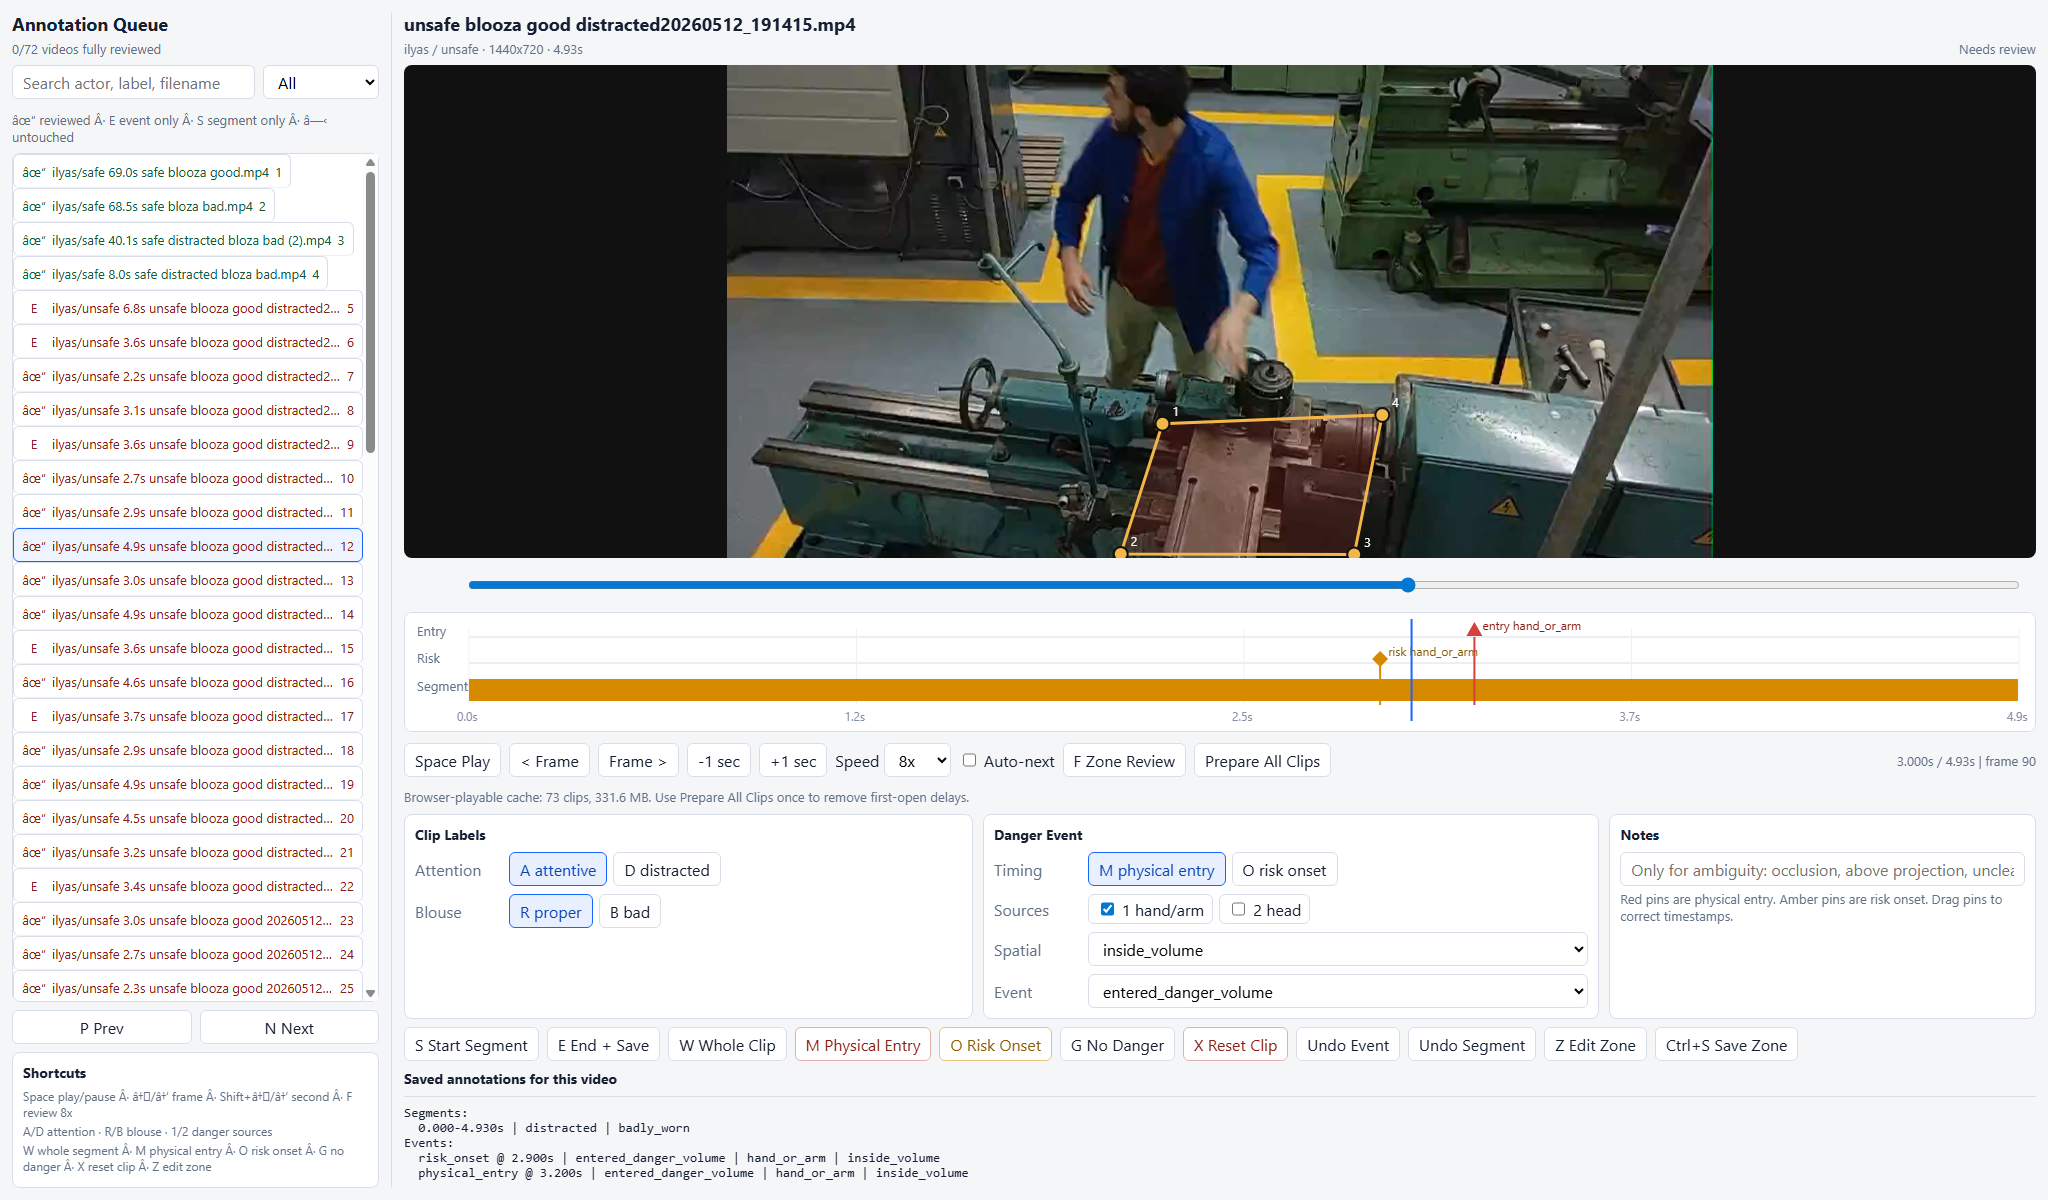
\includegraphics[width=0.98\linewidth]{figures/annotation_tool_interface.png}
\caption{Interface d'annotation développée pour le projet. Le polygone orange représente la zone dangereuse projetée, le marqueur ambre le début du risque, le marqueur rouge l'entrée physique, et la barre de segment stocke les labels attention/blouse.}
\end{figure}

\section{Chaîne de traitement et feature engineering}
Le pipeline ne donne pas les pixels bruts directement au modèle de danger principal. Chaque frame passe d'abord par YOLO pose, puis les points du corps sont comparés à la zone dangereuse annotée. Cette étape est une vraie étape de feature engineering: elle transforme une image en signaux structurés et interprétables sur la position et le mouvement du corps par rapport à la machine.

\begin{figure}[H]
\centering
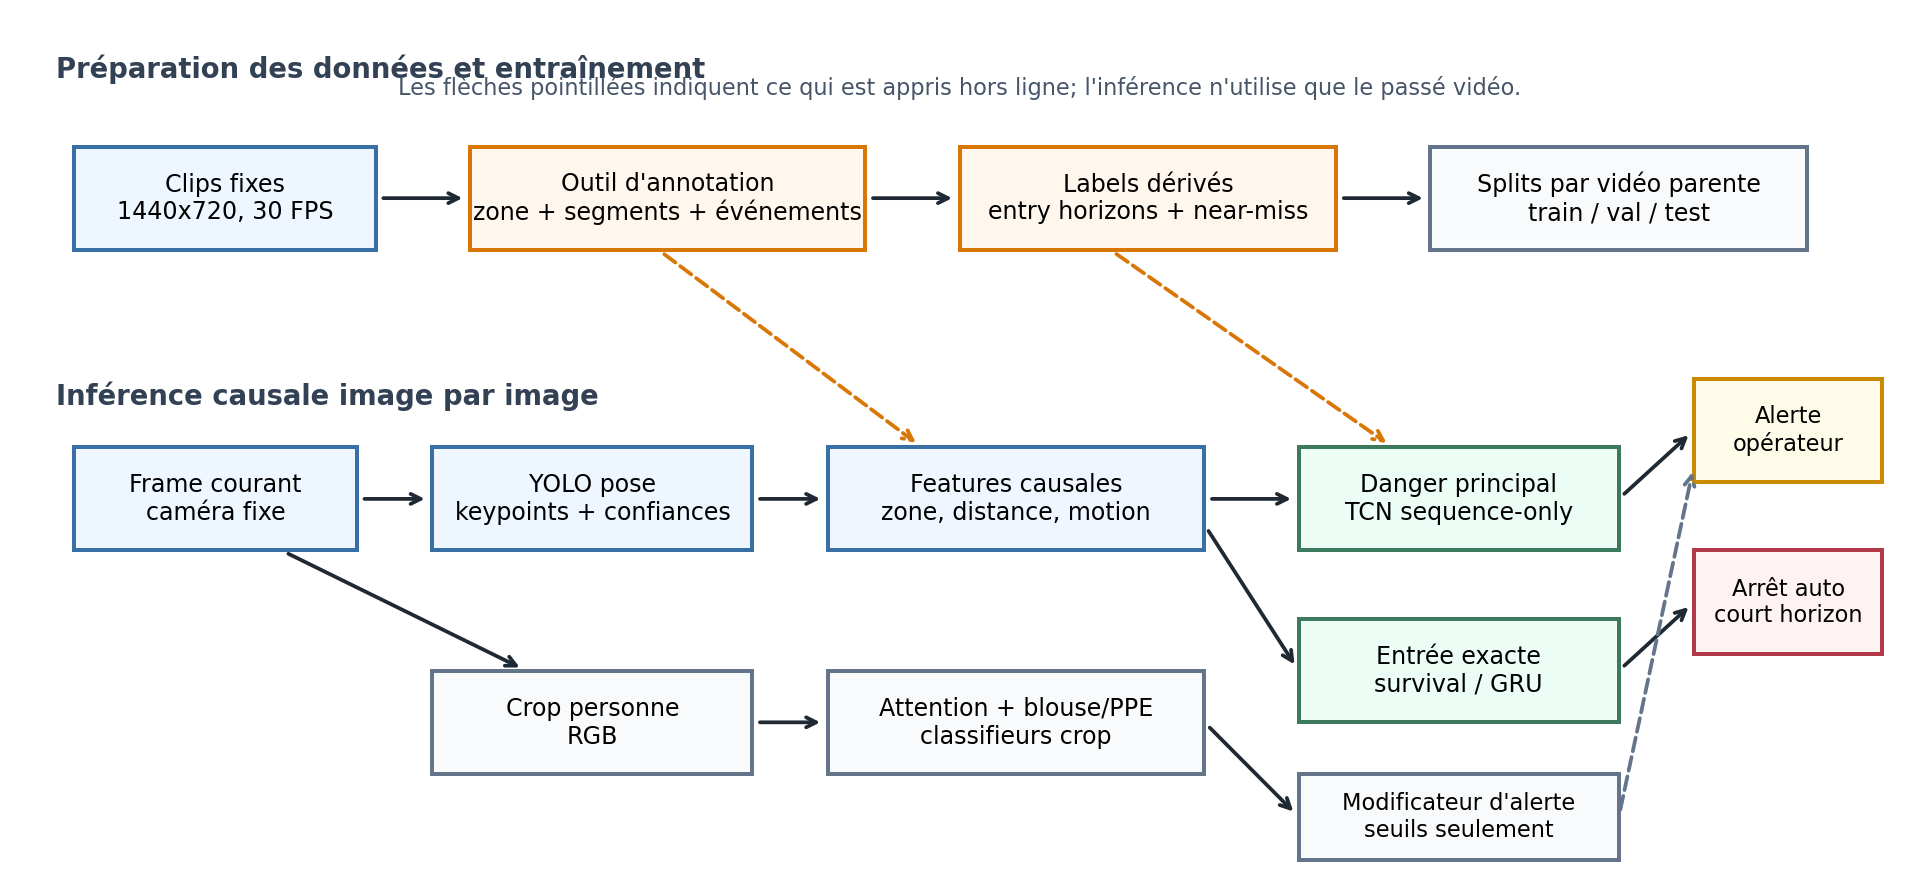
\includegraphics[width=0.95\linewidth]{figures/pipeline_policy_diagram.png}
\caption{Pipeline final utilisé dans le projet. L'annotation produit la zone, les segments et les événements qui servent à créer les labels; l'inférence temps réel passe par les features pose-zone causales, les modèles danger/entrée, puis les politiques d'alerte et d'arrêt.}
\end{figure}

\subsection{Features pose-zone causales}
Les features principales décrivent les poignets, coudes, tête et torse. Pour chaque partie utile du corps, on conserve des coordonnées normalisées, la confiance/visibilité de la pose, la distance signée à la zone dangereuse, un indicateur dedans/dehors, puis des dérivées temporelles comme la vitesse et l'accélération. Ces variables sont calculées sans regarder les frames futures: une fenêtre à l'instant $t$ contient seulement l'historique disponible jusqu'à $t$.

La projection 2D de la zone dangereuse est acceptable pour ce prototype parce que la caméra et la machine restent fixes, mais elle ne suffit pas pour un déploiement réel où la profondeur, les occlusions et les changements d'angle peuvent déplacer le corps par rapport au volume physique.

Ce choix rend le modèle plus interprétable qu'un classifieur d'image brut sur un petit dataset. Le modèle apprend principalement une dynamique de rapprochement vers la zone, au lieu de mémoriser l'arrière-plan, l'acteur, ou la couleur dominante d'une vidéo. Nous avons quand même testé des variantes de features et des contrôles négatifs, par exemple sans géométrie de zone, pour vérifier que la performance dépend bien de l'information pose-zone.

\section{Modèles}
Tous les modèles de danger restent évalués par rapport au même événement objectif: l'entrée physique d'une partie du corps dans la zone dangereuse. Pour l'alerte opérateur, nous avons cependant choisi une formulation plus directe qu'un horizon fixe: le modèle produit un seul score \texttt{risk\_present\_now}. Ce score veut dire: ``à cet instant, les indices pose-zone ressemblent déjà à une situation dangereuse visible''. Il ne prédit pas explicitement si l'entrée arrivera dans $0,5$ s ou $1,0$ s.

La supervision de ce score unique utilise nos annotations temporelles. Une fenêtre est positive entre \texttt{risk\_onset} et \texttt{physical\_entry}: c'est la période où un technicien ou un responsable sécurité pourrait raisonnablement commencer à voir le risque, mais avant l'entrée objective dans le volume dangereux. Ensuite, l'évaluation reste stricte: quand le score dépasse un seuil, on mesure si ce déclenchement arrive avant \texttt{physical\_entry}, puis combien de temps avant.

\subsection{Architectures du système}
Le système repose sur les mêmes variables d'entrée causales dans les deux cas: coordonnées de pose, visibilité, distances à la zone dangereuse, indicateurs d'intérieur de zone, vitesse et accélération. Nous distinguons ensuite deux usages opérationnels. Le TCN porte l'alerte opérateur avec un score unique de risque visible maintenant. Le GRU exact-entry sert le stop court horizon, quand la question devient celle de l'imminence de l'entrée physique à quelques dixièmes de seconde près.

\paragraph{TCN60 pour l'alerte opérateur.}
Le TCN60 reçoit une fenêtre causale de $60 \times 54$ features, soit environ deux secondes d'historique. Il applique une projection \texttt{Conv1d} $54 \rightarrow 96$, puis quatre blocs TCN résiduels avec dilatations $1,2,4,8$. Chaque bloc contient deux convolutions 1D, \texttt{BatchNorm}, \texttt{ReLU} et un dropout de $0,18$. La tête concatène la moyenne temporelle et le dernier pas temporel, puis applique un MLP $192 \rightarrow 96 \rightarrow 1$. La sortie unique est \texttt{risk\_present\_now}. Dans ce rapport, la politique d'alerte principale s'appuie sur la variante \texttt{tcn60\_aug\_bce}, parce qu'elle combine une avance utile et un bruit contenu.

\paragraph{GRU exact-entry comme signal d'arrêt court horizon.}
Le modèle GRU conservé pour l'arrêt automatique travaille sur une fenêtre causale plus courte et sur une cible plus stricte: non pas ``il y a un risque visible maintenant'', mais ``l'entrée physique est-elle devenue imminente?''. Dans le rapport, nous retenons son score \texttt{score\_by\_02}, c'est-à-dire le signal le plus proche de l'horizon $0,2$ s avant entrée. Ce GRU sert à auditer le compromis d'un signal de stop très tardif mais plus fiable à très courte échéance.

En résumé, le score principal ne demande pas au modèle de sortir un temps restant. Il demande seulement un niveau de certitude instantané sur la présence d'un risque visible. L'avance temporelle n'est pas une sortie du modèle: elle est mesurée après coup en comparant le premier déclenchement au temps réel d'entrée physique.

\subsection{Méthodes d'ensemble et fonctions de perte}
Pour la sortie unique \texttt{risk\_present\_now}, nous évaluons plusieurs variantes directes sur les mêmes splits répétés:
\begin{itemize}[leftmargin=*]
\item \texttt{tcn60\_aug\_bce}: TCN60 avec augmentation temporelle et perte BCE;
\item \texttt{tcn60\_aug\_focal}: TCN60 avec augmentation temporelle et perte focal.
\end{itemize}
En parallèle, le stop court horizon repose sur une expérience GRU exact-entry, évaluée comme signal d'imminence et non comme alerte opérateur.

Le terme \textbf{same-split} est important: les modèles combinés utilisent les mêmes séparations train, validation et test par vidéo parente. On ne mélange donc pas des prédictions venant de splits incompatibles, et on évite qu'une fenêtre d'une même vidéo aide indirectement à prédire une autre fenêtre de test. L'ensemble est volontairement simple: on moyenne les probabilités au lieu d'apprendre une fusion plus complexe. Ce choix réduit la variance sans ajouter beaucoup de paramètres, ce qui convient mieux à notre petit dataset.

\textbf{BCE} signifie \emph{Binary Cross Entropy}. C'est la perte standard pour une sortie binaire comme \texttt{risk\_present\_now}. Elle pénalise directement les erreurs entre la probabilité prédite et le label 0/1. Nous l'utilisons comme référence stable et facile à interpréter. Dans nos entraînements, elle est associée à un poids positif pour compenser le fait que les fenêtres positives sont beaucoup moins nombreuses que les fenêtres négatives.

\textbf{Focal loss} part de la BCE mais donne moins de poids aux exemples faciles et plus de poids aux exemples difficiles. Ici, cela aide parce que la majorité des fenêtres sont clairement négatives, alors que les fenêtres intéressantes sont proches de l'entrée et plus rares. Avec \texttt{gamma}=2, le modèle est poussé à mieux apprendre ces cas ambigus sans être dominé par les nombreux négatifs faciles.

\textbf{Augmentation temporelle} signifie que l'on perturbe légèrement les fenêtres temporelles pendant l'entraînement. Le but n'est pas de créer de nouveaux scénarios artificiels, mais d'éviter que le modèle mémorise un alignement exact de frames dans nos clips scénarisés. Le modèle doit apprendre une tendance causale de mouvement vers la zone, pas seulement reconnaître une position précise à une frame précise.

\subsection{Couche de politique: attention et blouse/PPE}
La sortie du modèle physique ne suffit pas à définir toute la politique d'usage. Deux situations peuvent justifier une alerte plus sensible: l'opérateur ne regarde pas correctement la zone de travail, ou la blouse/PPE est mal portée. Nous avons donc ajouté une couche de politique au-dessus du danger physique. Elle ne remplace pas le TCN/GRU et elle ne prétend pas prouver une cause physique d'entrée; elle pénalise seulement un contexte plus risqué.

On note $D$ le score de danger physique donné par le TCN60 \texttt{risk\_present\_now}, $A$ le score de risque attention, et $P$ le score de risque blouse/PPE. Les trois scores sont bornés entre 0 et 1. La politique finale conserve toujours le danger physique comme base:
\[
S_{\mathrm{sequence}} = D.
\]

La règle attention augmente le score si l'opérateur est distrait:
\[
S_{\mathrm{attention}} = 1 - (1-D)(1-0,30A).
\]
La règle blouse/PPE fonctionne de la même manière, avec un poids plus faible:
\[
S_{\mathrm{ppe}} = 1 - (1-D)(1-0,25P).
\]
La règle complète combine les deux pénalités contextuelles:
\[
S_{\mathrm{full}} = 1 - (1-D)(1-0,30A)(1-0,25P).
\]

Cette forme a deux propriétés utiles. Premièrement, si $A=0$ et $P=0$, alors $S_{\mathrm{full}}=D$: la couche de politique ne crée pas une alerte artificielle quand le contexte est normal. Deuxièmement, si le contexte devient mauvais, le score augmente mais reste borné par 1. En pratique, cela revient à baisser le seuil d'alerte quand le technicien est moins attentif ou moins protégé, tout en gardant l'arrêt automatique séparé de l'alerte opérateur.

Nous avons aussi testé des variantes plus sensibles, par exemple:
\[
S_{\mathrm{safety}} = 1 - (1-D)(1-0,45A)(1-0,35P),
\]
et une règle de haute sensibilité:
\[
S_{\mathrm{high}} = \mathrm{clip}\left(D + (1-D)(0,40A + 0,30P + 0,20AP), 0, 1\right).
\]
Ces variantes servent à explorer des politiques d'alerte plus sensibles. Dans notre lecture, attention et blouse/PPE modifient la sensibilité de l'alerte opérateur, mais le danger physique reste porté par la séquence pose-zone.

\subsection{Entraînement et résultats des modèles attention/blouse}
Les modèles attention et blouse/PPE sont entraînés sur des crops RGB de la personne, pas sur la séquence de pose complète. À partir des bounding boxes de pose, on extrait un crop autour de l'opérateur avec une marge de 12\%. Les crops sont pris environ toutes les 15 frames, avec un maximum de 24 crops par vidéo, puis redimensionnés en $224 \times 224$. Les labels viennent des segments annotés: \texttt{attention=distracted} devient la classe positive du modèle attention, et \texttt{blouse=badly\_worn} devient la classe positive du modèle blouse/PPE.

\begin{figure}[H]
\centering
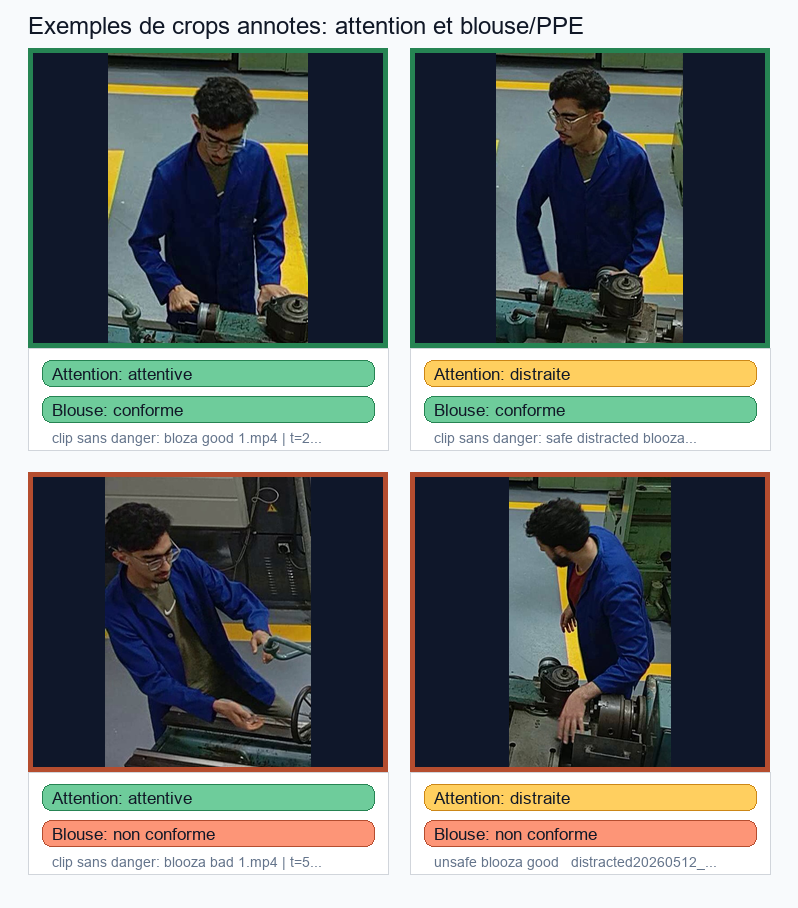
\includegraphics[width=0.86\linewidth]{figures/attention_blouse_examples.png}
\caption{Exemples de crops annotés utilisés pour les modèles attention et blouse/PPE. Chaque image garde le crop personne réellement extrait du dataset et affiche les deux labels de contexte qui alimentent la couche de politique.}
\end{figure}

Trois architectures ont été testées:
\begin{itemize}[leftmargin=*]
\item \texttt{small\_cnn}: petit CNN entraîné pour vérifier qu'un modèle simple suffit parfois;
\item \texttt{mobilenet\_v3\_small}: modèle léger pré-entraîné, utile pour un déploiement rapide;
\item \texttt{resnet18}: modèle pré-entraîné plus robuste, avec seulement les dernières couches adaptées.
\end{itemize}

L'entraînement utilise \texttt{BCEWithLogitsLoss} avec un poids positif pour compenser le déséquilibre entre classes. Les modèles sont entraînés avec \texttt{AdamW}, learning rate $3\cdot10^{-4}$, weight decay $10^{-4}$, batch size 32, early stopping sur l'AP validation, et augmentations d'image pendant l'entraînement: recadrage aléatoire, flip horizontal faible, jitter couleur, petite rotation et blur léger. L'évaluation finale est faite au niveau vidéo: les scores de crop sont moyennés par vidéo parente, puis comparés au label vidéo. Cela évite de présenter plusieurs crops voisins comme des exemples indépendants.

\begin{table}[H]
\centering
\caption{Résultats crop CNN sur 20 splits répétés, au niveau vidéo test. AP = average precision. BA = balanced accuracy.}
\resizebox{\linewidth}{!}{%
\begin{tabular}{llrrrr}
\toprule
Tâche & Meilleure architecture & AP & ROC AUC & F1 & BA \\
\midrule
Attention distraite & \texttt{resnet18} & 0.921 & 0.914 & 0.898 & 0.914 \\
Blouse/PPE mal porté & \texttt{resnet18} & 0.985 & 0.982 & 0.974 & 0.965 \\
\bottomrule
\end{tabular}
}
\end{table}

Les résultats montrent deux niveaux de confiance différents. Le signal blouse/PPE est le plus fort: les formes et couleurs de la tenue sont visibles dans le crop, et les résultats restent très élevés sur les splits répétés. Le signal attention est exploitable mais moins robuste: il dépend davantage de la pose de la tête, de l'orientation du corps et du cadrage. Les tests d'augmentation confirment aussi cette différence: la blouse/PPE est presque saturée dans plusieurs politiques d'augmentation, alors que l'attention bénéficie d'augmentations modérées et reste plus variable.

Nous avons également testé un actor-holdout, où un acteur est retiré de l'entraînement et utilisé comme test. Dans ce cas, les performances baissent, surtout pour l'attention. Par exemple, les meilleurs scores attention restent autour de $0,80$ de balanced accuracy selon l'acteur placé en test, tandis que blouse/PPE varie davantage entre acteurs. Cela confirme que ces modèles sont utiles comme contexte de politique, mais pas assez validés pour remplacer le modèle physique de danger.

\section{Protocole d'évaluation}
L'évaluation est causale: à l'instant $t$, aucune image future n'est utilisée. Les splits sont faits par vidéo parente pour éviter la fuite de données entre fenêtres voisines. Comme le dataset reste petit, nous n'avons pas voulu fonder l'analyse sur une seule séparation train/validation/test. Nous avons donc utilisé des splits répétés avec différentes graines aléatoires: chaque répétition garde l'étanchéité par vidéo parente, puis les métriques sont agrégées. Cette stratégie ne remplace pas un dataset plus grand, mais elle réduit la dépendance à un split chanceux ou défavorable et donne une estimation plus robuste de la variabilité expérimentale. L'entrée physique reste la référence quantitative principale, mais le \texttt{risk\_onset} sert de repère humain: une bonne alerte doit être assez tôt pour se rapprocher de ce qu'un expert verrait avant l'accident, sans multiplier les faux positifs. Les métriques utilisées sont:
\begin{itemize}[leftmargin=*]
\item \textbf{hit}: le modèle déclenche au moins une fois avant l'entrée physique;
\item \textbf{early 0,2/0,3}: le premier déclenchement arrive au moins ce nombre de secondes avant l'entrée;
\item \textbf{précision}: proportion des alarmes qui correspondent à un vrai événement;
\item \textbf{FA/min}: faux positifs par minute;
\item \textbf{fiabilité court horizon}: quand le score est très haut, probabilité empirique que l'entrée arrive vite.
\end{itemize}

\section{Expériences menées}
Les expériences suivent une logique progressive. Nous avons d'abord testé des baselines tabulaires sur fenêtres de features agrégées, afin de vérifier que les distances à la zone et les vitesses contenaient déjà un signal. Nous avons ensuite entraîné des modèles séquentiels plus adaptés au caractère temporel du problème: TCN, CNN1D, GRU, LSTM et Transformers, avec plusieurs longueurs de fenêtre. La politique d'alerte décrite dans ce rapport repose ensuite sur une sortie unique, \texttt{risk\_present\_now}. Les modèles décrits ici respectent tous le protocole causal et les splits par vidéo parente.

Plusieurs ablations ont servi à clarifier ce que le modèle apprenait réellement:
\begin{itemize}[leftmargin=*]
\item \textbf{features}: comparaison entre toutes les features, features main/bras, features tête/torse, et versions sans géométrie de zone;
\item \textbf{pertes}: BCE pondérée contre focal loss, pour tester la robustesse au déséquilibre positif/négatif;
\item \textbf{augmentation}: bruit léger sur les features, perturbations temporelles, dropout de pose et variations de vitesse;
\item \textbf{sortie unique}: sélection du TCN60 sur la cible \texttt{risk\_present\_now}, puis mesure de l'avance réelle sur \texttt{physical\_entry};
\item \textbf{stop court horizon}: audit séparé du \texttt{survival\_gru\_exact\_entry} avec le score \texttt{score\_by\_02}, centré sur l'imminence à $0,2$--$0,3$ s;
\item \textbf{généralisation}: splits répétés et actor-holdout, afin de mesurer la sensibilité aux deux acteurs du dataset;
\item \textbf{contexte}: modèles crop séparés pour attention et blouse/PPE, utilisés ensuite seulement dans la couche de politique.
\end{itemize}

Cette sélection évite de présenter un seul chiffre isolé. Le résultat final est choisi parce qu'il reste cohérent avec la contrainte causale, la séparation par vidéo parente et l'objectif opérationnel visé.

\section{Résultats principaux}
\begin{table}[H]
\centering
\caption{Alerte opérateur: trade-off interne du TCN à sortie unique sur splits de test répétés.}
\resizebox{\linewidth}{!}{%
\begin{tabular}{lrrrrr}
\toprule
Politique & Early 0,2 & Early 0,3 & Précision & FA/min & Lead médian \\
\midrule
TCN60, seuil 0,55 & 0.850 & 0.642 & 0.859 & 1.574 & 0.394 s \\
TCN60, seuil 0,35 & 0.850 & 0.683 & 0.661 & 6.015 & 0.456 s \\
\bottomrule
\end{tabular}
}
\end{table}

Cette table présente deux points de fonctionnement du TCN d'alerte. Le seuil $0,55$ correspond à une alerte opérateur continue où l'avance utile reste élevée et le bruit contenu. Le seuil $0,35$ gagne légèrement à $0,3$ s, mais au prix d'une hausse marquée des fausses alertes.

\reportnote{SoftBlue}{\textbf{Interprétation.} La sortie du modèle n'est pas un compte à rebours. C'est un score de certitude instantané. Les colonnes Early 0,2 et Early 0,3 sont calculées après coup: elles disent combien de déclenchements arrivent au moins 0,2 s ou 0,3 s avant l'entrée physique.}

\section{Signal d'arrêt automatique}
Le score \texttt{risk\_present\_now} est une alerte opérateur. Pour discuter un arrêt automatique, nous utilisons séparément le GRU exact-entry court horizon \texttt{survival\_gru\_exact\_entry}. Ici, la question n'est plus ``l'alerte est-elle assez tôt pour un humain?'', mais ``quand le signal de stop se déclenche, l'entrée physique est-elle réellement imminente à $0,2$--$0,3$ s près?''.

\begin{table}[H]
\centering
\caption{GRU exact-entry: trade-off du signal de stop court horizon.}
\resizebox{\linewidth}{!}{%
\begin{tabular}{lrrrrr}
\toprule
Signal & Fenêtres déclenchées & $P(\mathrm{entree}\le0,2s)$ & $P(\mathrm{entree}\le0,3s)$ & Temps moyen avant entrée \\
\midrule
GRU exact-entry strict, seuil 0,95 & 16 & 0.708 & 0.903 & 0.133 s \\
GRU exact-entry plus couvrant, seuil 0,90 & 51 & 0.502 & 0.741 & 0.221 s \\
\bottomrule
\end{tabular}
}
\end{table}

Cette table ne mesure pas si tous les clips dangereux sont couverts. Elle pose la question inverse: quand le signal de stop se déclenche, l'entrée physique est-elle réellement imminente? Le seuil $0,95$ donne la lecture la plus stricte: moins de déclenchements, mais une bien meilleure probabilité d'être vraiment à moins de $0,2$--$0,3$ s de l'entrée. Le seuil $0,90$ est plus couvrant et part un peu plus tôt, mais il perd nettement en fiabilité. Le compromis se lit donc à l'intérieur de la logique d'arrêt elle-même.

Cette analyse reste secondaire dans ce rapport. Elle est utile pour discuter l'arrêt machine, mais elle est trop tardive pour une réaction humaine confortable.

\section{Temps réel}
Le chemin vidéo brut avec extraction de pose mesure 33.20 ms/image en moyenne et 38.39 ms/image au p95. Le TCN lui-même est négligeable par rapport à l'extraction de pose. Pour un signal moyen à 133 ms avant l'entrée, il reste environ 99.8 ms avec la latence moyenne, ou 94.6 ms avec la latence p95, pour l'électronique et la mécanique.

\begin{figure}[H]
\centering
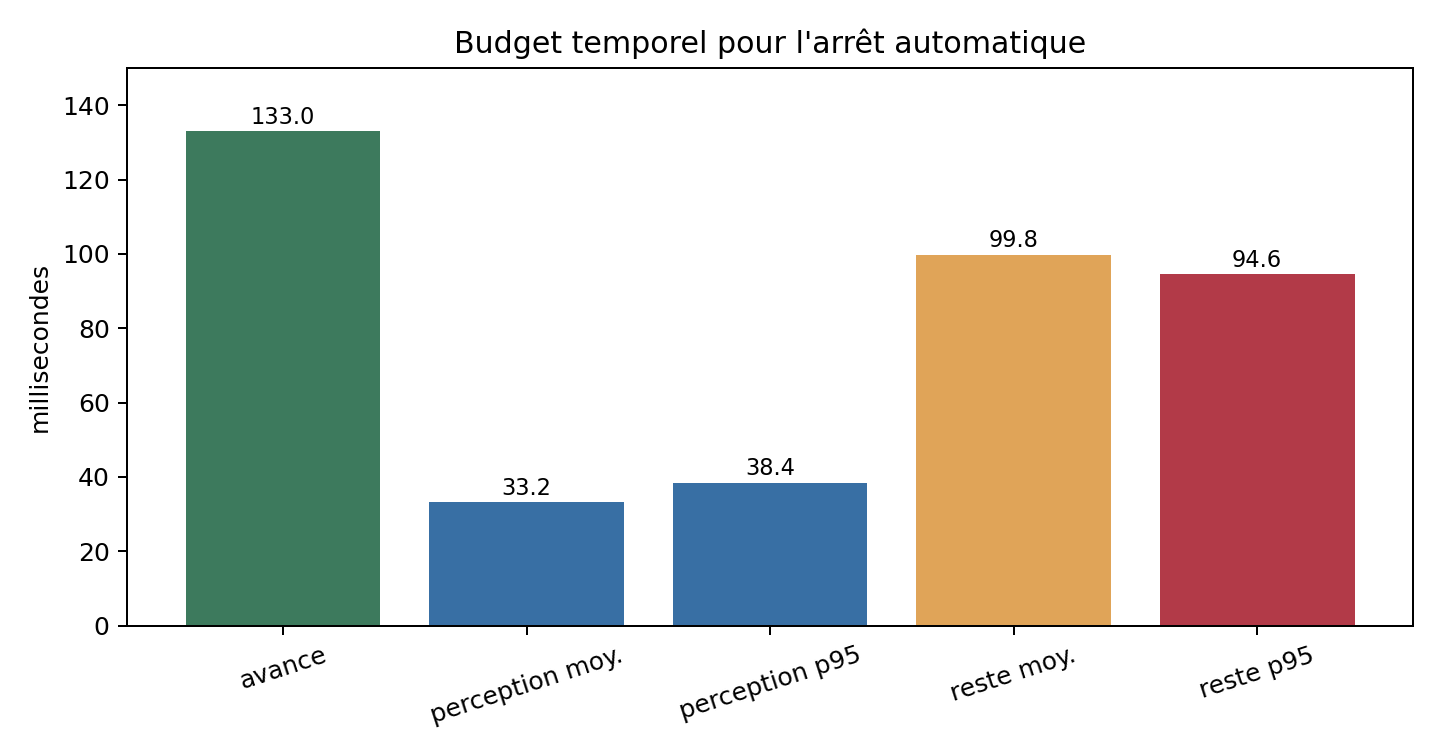
\includegraphics[width=0.80\linewidth]{figures/timing_budget.png}
\caption{Budget temporel approximatif pour l'arrêt automatique.}
\end{figure}

\section{Discussion}
Le point central du projet est la séparation entre prédire un risque et décider une action. Le modèle principal ne prédit pas un compte à rebours. Il dit seulement que, maintenant, la dynamique pose-zone ressemble à un risque visible. Ensuite, l'audit mesure si ce déclenchement arrive assez tôt avant l'entrée physique. Cette formulation évite de surinterpréter des horizons comme \texttt{danger\_within\_0.5s}: dans notre cas, ce label signifie bien ``entrée physique dans $0,5$ s'', mais la politique d'alerte se base sur un score unique de risque présent.

La couche attention/blouse doit aussi être interprétée comme une couche de politique. Elle ne dit pas qu'une mauvaise blouse ou un regard détourné causent l'entrée dans la zone. Elle dit seulement que, si le danger physique est déjà non nul, le système peut devenir plus sensible lorsque le contexte humain est moins favorable. Cette distinction évite de transformer des corrélations d'un petit dataset en conclusion causale trop forte.

Enfin, les annotations de \texttt{risk\_onset} donnent un repère humain utile pour raconter l'anticipation, mais elles ne remplacent pas l'entrée physique comme vérité terrain principale. La cible objective reste le moment où le corps entre dans le volume dangereux.

\section{Limites}
Le dataset est petit, scénarisé, avec deux acteurs, une seule machine et une seule caméra. Le résultat est donc un prototype académique, pas une validation industrielle certifiable. La projection 2D de la zone dangereuse est acceptable ici parce que la caméra et la machine restent fixes, mais elle ne suffit pas pour un déploiement où la profondeur réelle, les occlusions et les changements d'angle peuvent modifier la position du corps par rapport au volume dangereux. Les modèles attention/PPE sont utiles pour la politique d'alerte, mais leur généralisation reste limitée. Un déploiement réel demanderait plus d'acteurs, plus de vrais négatifs, une mesure de la chaîne d'arrêt complète et une validation de sécurité formelle.

\section{Conclusion}
Le projet atteint plusieurs résultats importants. D'abord, il montre qu'une caméra fixe peut fournir un signal exploitable avant l'entrée physique dans une zone dangereuse, sans utiliser d'images futures. Le modèle \texttt{tcn60\_aug\_bce} donne une base claire pour l'alerte opérateur: avec un seul score \texttt{risk\_present\_now}, il atteint $0,850$ de détection au moins $0,2$ s avant l'entrée, $0,642$ à $0,3$ s, une précision de $0,859$ et $1,574$ fausse alerte/min sur les splits de test répétés. Pour l'arrêt court horizon, le GRU exact-entry apporte une information différente: au seuil strict observé, il donne $P(\mathrm{entree}\le0,2s)=0.708$ et $P(\mathrm{entree}\le0,3s)=0.903$, avec un temps moyen avant entrée de $0,133$ s. Le rapport distingue donc bien deux usages: le TCN pour l'alerte opérateur continue, le GRU pour l'audit d'un signal de stop imminent.

Un autre gain concret est méthodologique. Le projet ne se limite pas à entraîner un modèle: il construit une chaîne complète, depuis l'annotation de la zone et des événements jusqu'aux features causales, aux modèles séquentiels, aux politiques d'alerte et à l'audit de latence. L'outil d'annotation développé pour le projet a permis de séparer l'entrée physique, qui reste la vérité terrain objective, du risque visible humain, qui sert à raisonner sur l'anticipation attendue par un technicien ou un responsable sécurité. Les modèles attention et blouse/PPE ajoutent aussi une dimension utile: ils ne remplacent pas le danger physique, mais ils permettent d'ajuster la sensibilité de l'alerte quand le contexte humain devient moins favorable.

Les prochaines étapes sont claires. Il faudrait collecter plus de vidéos avec plus d'acteurs, plus de vrais négatifs, plusieurs machines et plusieurs angles de caméra, idéalement avec une vue multi-angle ou une information de profondeur. Il faudrait aussi mesurer la chaîne d'arrêt complète, de la capture vidéo jusqu'à l'action mécanique, afin de vérifier si la marge temporelle observée suffit réellement en conditions physiques. Enfin, une version industrielle devrait intégrer une validation 3D plus robuste de la zone dangereuse, une calibration caméra plus formelle, et une évaluation de sûreté séparée du simple score de classification.

\end{document}
